\section{Swarm analysis}
\label{sec:swarm}

%\subsection{Consensus of a swarm}

%\begin{itemize}
%\item Combinations of ISS parts are ISS
%\item Swarm as such a combination
%\item Conditions where update is ISS
%\item trivially at stagnation. But also when on a single hill
%\end{itemize}

%\begin{itemize}
%\item Bound on swarm for the single hill case (perhaps as function of the width of the hill?
%Or width of the hill as a percentage of the feasible region?)
%\item test on 2-d case to show that the bound can prevent a particle from reaching another hill.
%This is one form of the swarm failing to converge the global optimal.
%\item Can we look at parameters for the whole swarm?
%\end{itemize}

In section \ref{sec:particle}, we can see the limitation of the search capacity of a particle.
The particle is in a randomized walk in an attractive potential fields defined by the global best and the personal best.
There exists a lot of factors that prevents the particle reaching the optimal.
The swarm initializes the particles randomly in the search space and has the particles searching the optimal simultaneously, which forms a beam-search style.
The import of interaction topology enhances the search capability, which makes it more than a beam-search style optimization method.
In this section, we analyze the star topology of global best update.
In this topology, the global best update imports the competition among the particles.
The particle finds a new global best becomes the leader of the swarm.

\subsection{Unimodal fitness distribution}

Due to the potential competition in the swarm, if there is always a particle finds a better solution till the optimal is reached, the swarm can always find the optimal in the unimodal case.
We have Theorem \ref{thm:singleHill:swarm:converge}.

\begin{mythm}
\label{thm:singleHill:swarm:converge}
In the unimodal case, when there are more than two particles, $ x^{G} \rightarrow x^{*} $ if all the particles has input-to-state stable position update component.
\begin{proof}
There are two cases, $ x^{G} = x^{*} $ and $ x^{G} \not = x^{*} $
If the global best is $ x^{*} $, the particles will gradually converge to $ x^{*} $ by Lemma \ref{lem:singleHill:particle:nonstop}.
If the global best is not $ x^{*} $, the particles will take turns to find new global best by Theorem \ref{thm:singleHill:particle:better} till $ x^{*} = x^{G} $.
Then it becomes the case $ x^{G} = x^{*} $.
\end{proof}
\end{mythm}

%[TODO:] More particles --> convergence rate
%This is hard. Because convergence rate is not a constant.

%\subsubsection{Simulation}

\subsection{Multi-modal fitness distribution}

When the fitness distribution is not unimodal, there exists more varieties in the movement patterns of the particles.
The probability that a particle find a new global best depends on the position, the personal best and the fitness distribution near around.
The increase of the number of the particles raise the probability that the swarm can find a new global best.
We have Theorem \ref{thm:nonsingleHill:swarm:prob}.

\begin{mythm}
\label{thm:nonsingleHill:swarm:prob}
The probability that the swarm finds a better global best depends on the probabilities that the particles find better global best, which is
\begin{equation}
\label{eq:prob_sum}
P = 1 - \prod_{i=1}^{N} ( 1 - P_{i} ),
\end{equation}
$ P_{i} $ is the probability of particle $ i $ finds a new global best
and $ P $ is the probability that the swarm finds a new global best.
\begin{equation}
\label{eq:prob_less}
\forall i \in [1, N], P_{i} < P.
\end{equation}
\begin{proof}
The search process is a competition among the particles in the swarm.
If the swarm does not find a better global best, it means that none of the particle finds a better global best.
For particle $ i $, the probability that a new global best cannot be found is $ 1 - P_{i} $.
Because the global best is constant, the movements of the particles are independent in the search process.
Thus, the probability that no particle finds a new global best becomes
$ \prod_{i=1}^{N} ( 1 - P_{i} ) $.
Then we can know that the probability that a new global best can be found by the swarm.
By writing Equation \ref{eq:prob_sum} as $ P = 1 - ( 1 - P_{i} ) \prod_{j=1, j \not = i}^{N}  ( 1 - P_{j} ) $ and $ \prod_{j=1, j \not = i}^{N}  ( 1 - P_{j} ) \leq 1 $,
we have Equation \ref{eq:prob_less}.
\end{proof}
\end{mythm}

\begin{figure}
\centering
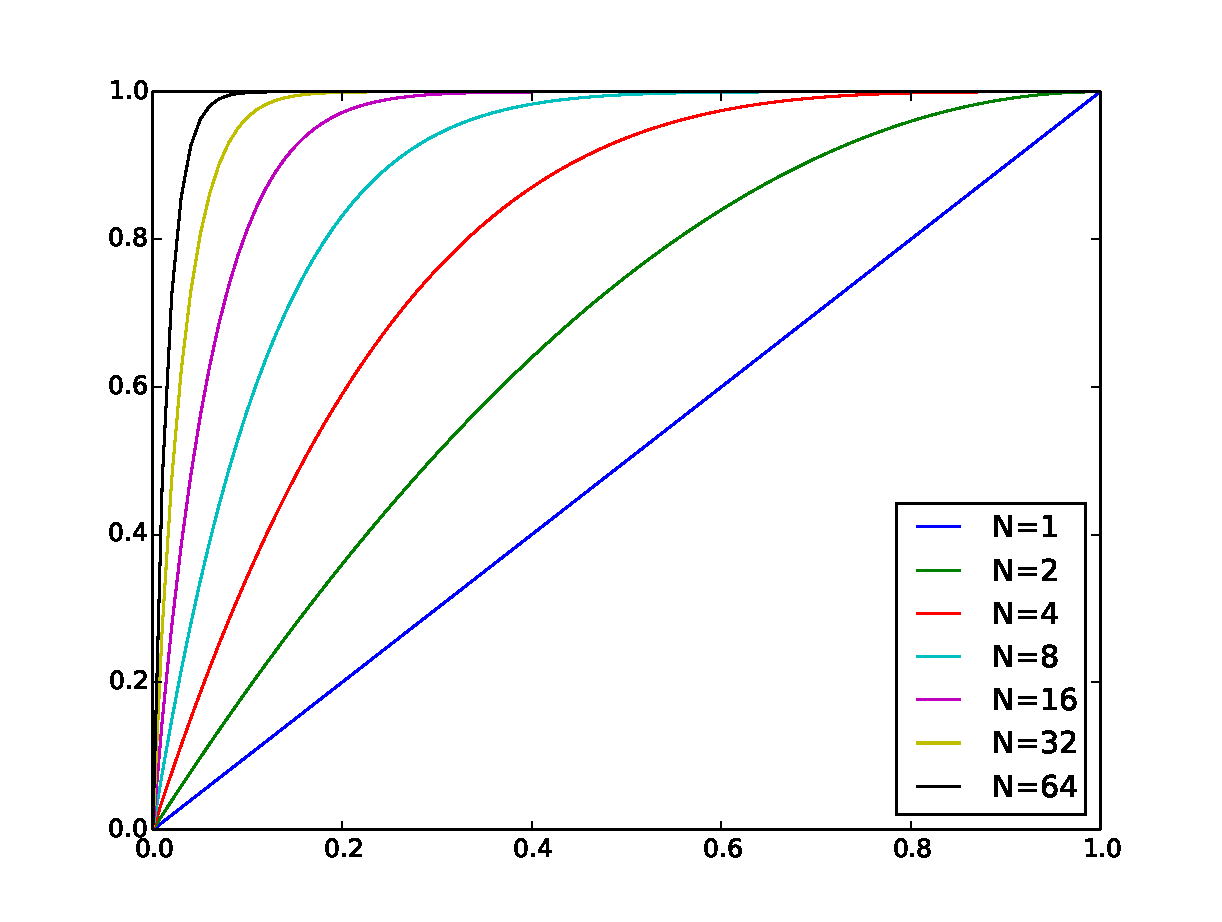
\includegraphics[width=0.7\linewidth]{./fig/probRise}
\caption{The probability increases with the particle number.}
\label{fig:probRise}
\end{figure}

Figure \ref{fig:probRise} illustrates how the probability of the swarm increases with the number of the particles, assuming that the probabilities of all the particles are the same.
The uniformly random initialization enables the diversity of the probabilities of the particles, which should increase the probability of the swarm as well.


%\subsubsection{Simulation}

\subsection{Value of a swarm}

%Being on one hill is the unlikely case bound in the multi hill case.
%Might not seem useful but is the essence of what makes a swarm a swarm.
%Bounds the swarm to a region around p-bests where g-best has been unable to pull other particles to its hill.
%For a function with narrow hills, g-bests on a narrow hills is less likely to capture another particle, thus the swarm searches more, for functions with broad hills, p-gest are more likely to be pulled to g-bests hill and search there.
%Thus swarm diversity is the mechanism that allows the swarm to not converge when searching is likely needed but focus and converge when the fitness landscape appear to favor exploitation.
%This does not happen at stagnation and does not happen without multiple members. <need to say this in a more mathematical way>>

%example ?? function for exploration case
%example sphere function for the exploitation case
%try to use bound as a function of hill width metric

%Rastrigin as a counter example? Does it get stuck or just sample for ever? It certainly runs longer.

\subsubsection{Competition}

\begin{itemize}
\item The existence of a competition enhances the chance that the global best can be refined, which increases the probability that the global optimal can be found.
\item 
\item 
\end{itemize}

\subsubsection{Diversity}

\begin{itemize}
\item The uniformly initialization on the search space increases the inconsistency between the personal best and the global best.
It means that the particle moves in a larger range.
With a reasonable step length determined by $ \chi $, it is more likely to find a better solution.
\end{itemize}

\subsection{Diversity injection}

%Work with the Rastrigin function has lead others to experiment with diversity injection to prevent pre-mature convergence (or prevent convergence at all)
%I am not sure, do we want it to converge? ever?
%On what basis would I propose a new algorithm?
%Show that it would converge based on ISS?